\begin{textblock}{15.}(0., -2.)
    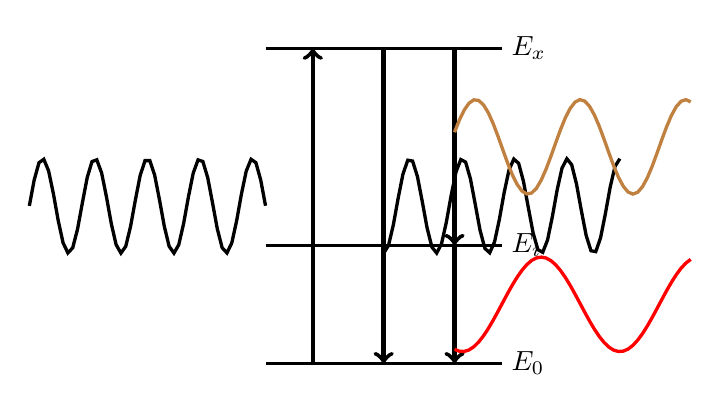
\begin{tikzpicture}
        %%% Definitions
        %% Mathematical constants
        \def \NWAVEFORMSAMPLES {50}

        %% Colors
        \def \INELASTICHIGHCOLOR {brown}
        \def \INELASTICLOWCOLOR {red}

        %% Incoming EM wave
        \def \AMPLITUDE {0.6}
        \def \WAVEFORMLENGTH {3.}
        \def \INWAVESTART {0.}
        \def \INWAVELENGTH {0.5}

        %% Outgoing EM wave
        \def \OUTWAVELENGTHHIGH {1.0}
        \def \OUTWAVELENGTHLOW {1.5}

        %% States
        \def \GROUNDSTATEY {-2.}
        \def \INTERMEDIATESTATEY {-0.5}
        \def \EXCITEDSTATEY {2.}
        \def \STATEXSTART {3.}
        \def \STATEX {3.}

        %% Transitions
        \def \EXCITATIONX {\STATEXSTART+0.2*\STATEX}
        \def \ELASTICX {\STATEXSTART+0.5*\STATEX}
        \def \INELASTICX {\STATEXSTART+0.8*\STATEX}

        %%% Drawing
        %% Incoming EM wave
        \draw [very thick, \ORANGE, domain=\INWAVESTART:\INWAVESTART+\WAVEFORMLENGTH, samples=\NWAVEFORMSAMPLES] plot (\x, {\AMPLITUDE*sin(\WAVEFORMLENGTH/\INWAVELENGTH*2*pi/4*\x r)});

        %% States
        % Ground state
        \draw[very thick, black] (\STATEXSTART, \GROUNDSTATEY) -- (\STATEXSTART+\STATEX, \GROUNDSTATEY);
        \draw (\STATEXSTART + \STATEX, \GROUNDSTATEY) node[anchor=west] {$E_0$};

        % Intermediate state
        \draw[very thick, black] (\STATEXSTART, \INTERMEDIATESTATEY) -- (\STATEXSTART+\STATEX, \INTERMEDIATESTATEY);
        \draw (\STATEXSTART + \STATEX, \INTERMEDIATESTATEY) node[anchor=west] {$E_i$};

        % Excited state
        \draw[very thick, black] (\STATEXSTART, \EXCITEDSTATEY) -- (\STATEXSTART+\STATEX, \EXCITEDSTATEY);
        \draw (\STATEXSTART + \STATEX, \EXCITEDSTATEY) node[anchor=west] {$E_x$};

        %% Transitions
        % Excitation
        \draw[->, ultra thick, black] (\EXCITATIONX, \GROUNDSTATEY) -- (\EXCITATIONX, \EXCITEDSTATEY);

        % Direct ground-state decay
        \visible<2->{
            \draw[->, ultra thick, black] (\ELASTICX, \EXCITEDSTATEY) -- (\ELASTICX, \GROUNDSTATEY);

            \draw [very thick, \ORANGE, domain=\ELASTICX:\ELASTICX+\WAVEFORMLENGTH, samples=\NWAVEFORMSAMPLES] plot (\x, {\AMPLITUDE*sin(\WAVEFORMLENGTH/\INWAVELENGTH*2*pi/4*\x r)});
        }

        % Decay via intermediate states
        \visible<3>{
            \draw[->, ultra thick, black] (\INELASTICX, \EXCITEDSTATEY) -- (\INELASTICX, \INTERMEDIATESTATEY);

            \draw [very thick, \INELASTICHIGHCOLOR, domain=\INELASTICX:\INELASTICX+\WAVEFORMLENGTH, samples=\NWAVEFORMSAMPLES] plot (\x, {\AMPLITUDE*sin(\WAVEFORMLENGTH/\OUTWAVELENGTHHIGH*2*pi/4*\x r) + \INTERMEDIATESTATEY + 0.5*(\EXCITEDSTATEY-\INTERMEDIATESTATEY)});

            \draw[->, ultra thick, black] (\INELASTICX, \INTERMEDIATESTATEY) -- (\INELASTICX, \GROUNDSTATEY);

            \draw [very thick, \INELASTICLOWCOLOR, domain=\INELASTICX:\INELASTICX+\WAVEFORMLENGTH, samples=\NWAVEFORMSAMPLES] plot (\x, {\AMPLITUDE*sin(\WAVEFORMLENGTH/\OUTWAVELENGTHLOW*2*pi/4*\x r) + \GROUNDSTATEY + 0.5*(\INTERMEDIATESTATEY-\GROUNDSTATEY)});
        }
    \end{tikzpicture}
\end{textblock}